% +-----+
% | A.1 |
% +-----+
\section{[Autofocus problems]}
\label{sec:A.1_title}

Acquisition of in-focus fluorescence microscopy (FM) images comprises an essential aspect of the workflow for integrated array tomography. Focusing the objective lens of the fluorescence microscope can be done manually or by an autofocus routine implemented in the microscope control software, Odemis.\footnote{\href{https://github.com/delmic/odemis}{https://github.com/delmic/odemis}} It was observed, however, that the autofocus routine is susceptible to errors (Figure \ref{fig:A.1_afruns}), even when initiated with seemingly favorable initial conditions. The routine works by acquiring and assessing the focus level of fluorescence images in an iterative fashion. The first image is acquired at the starting position of the objective lens, after which the lens is translated upwards and downwards by a fixed amount. At each position the focus level is measured by the variance of Laplacian. The objective is then iteratively translated upwards or downwards depending on whether the focus level improves or worsens. This iterative routine [makes sense conceptually, but runs into issues when the measurement is not reproducible when the objective returns to its original position] or if the focus evaluation metric (in this case the variance of Laplacian) is biased towards either over-focus or under-focus images.

% --- Fig A.1 (AF runs) ---
\begin{figure}[!tbh]
    \centering
    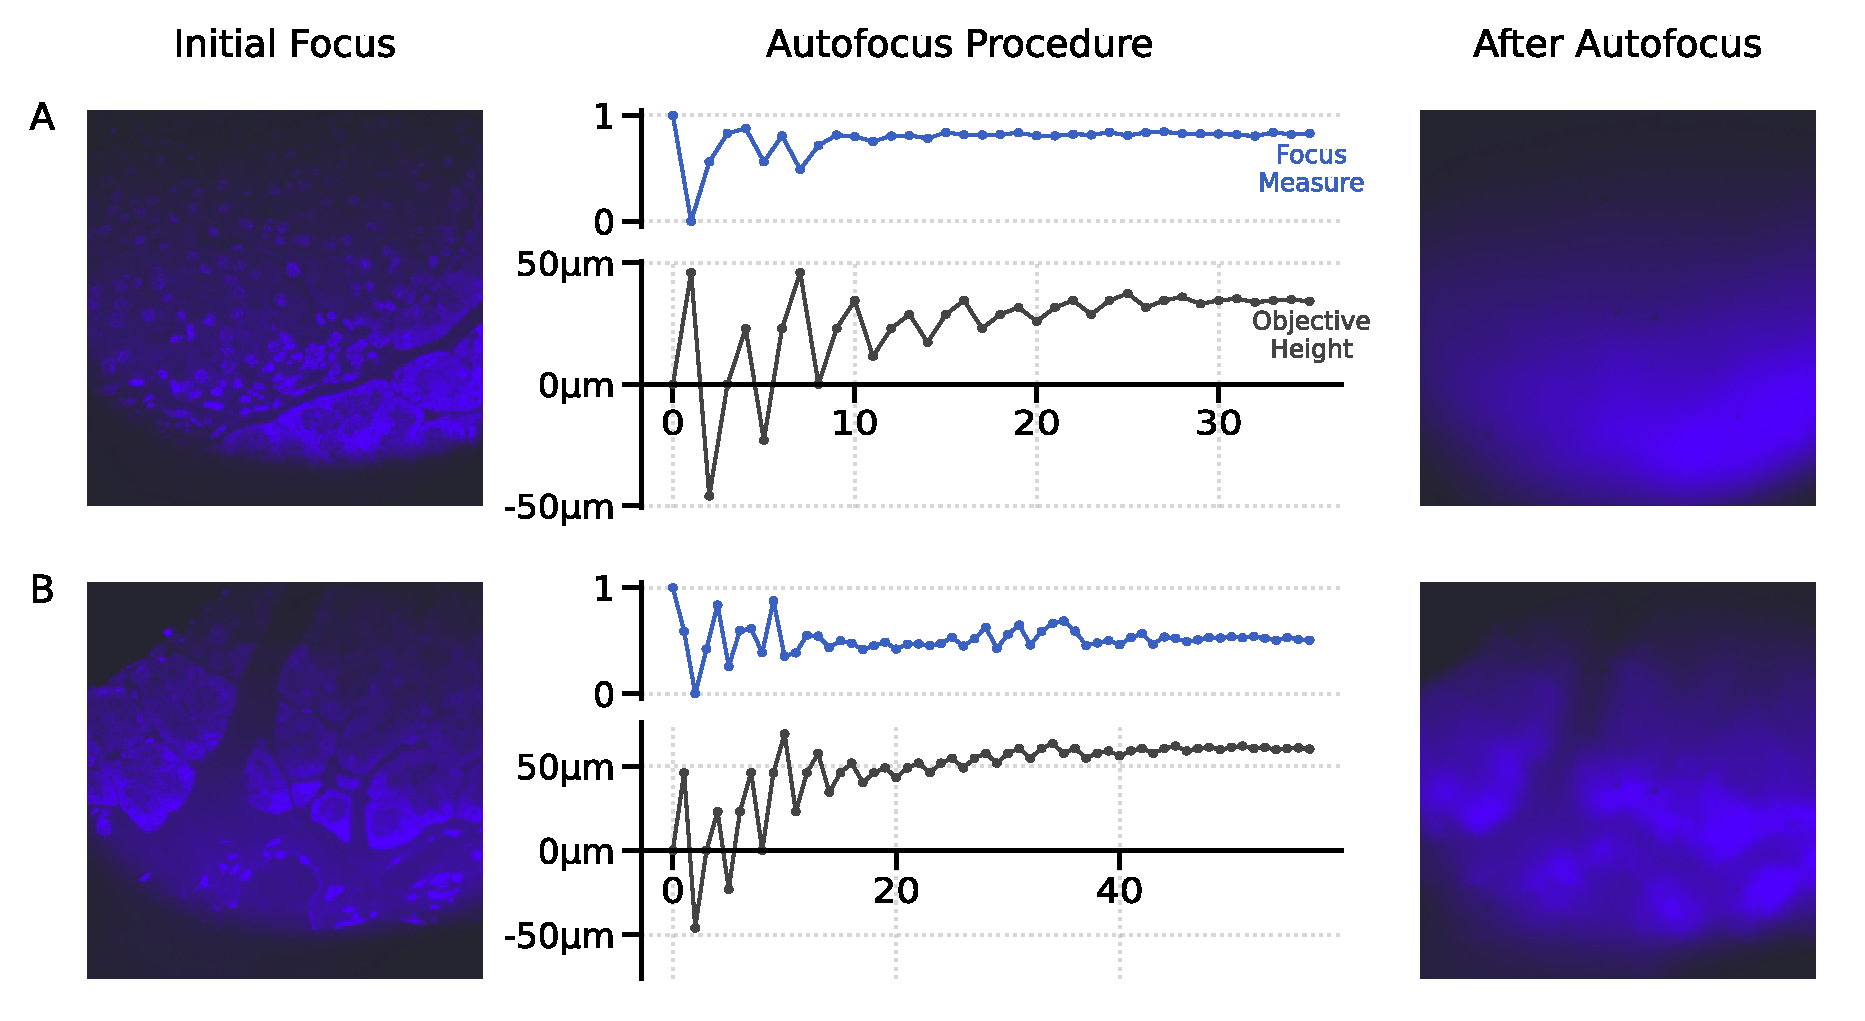
\includegraphics[width=\linewidth]{cppendix-A/figures/fig1_afruns_v3.pdf}
    \caption{Sample FM focus sweeps. x axis is iteration number}
    \label{fig:A.1_afruns}
\end{figure}


% +-----+
% | A.2 |
% +-----+
\section{Analysis of FM focus sweeps for autofocus algorithm selection}

Results in Fig A.1 / problems with autofocus suggest that the iterative nature of the autofocus routine is a possible failure mechanism as is the use of the variance of Laplacian as a focus measure. To further probe where the problem may lie / to try and possibly develop a better autofocus algorithm, we conduct a series of focus sweeps over a range of different ranges, and both fluorescence channels (Figure \ref{fig:A.2_sweeps}).

% --- Fig A.2 (sweeps) ---
\begin{figure}[!tbh]
    \centering
    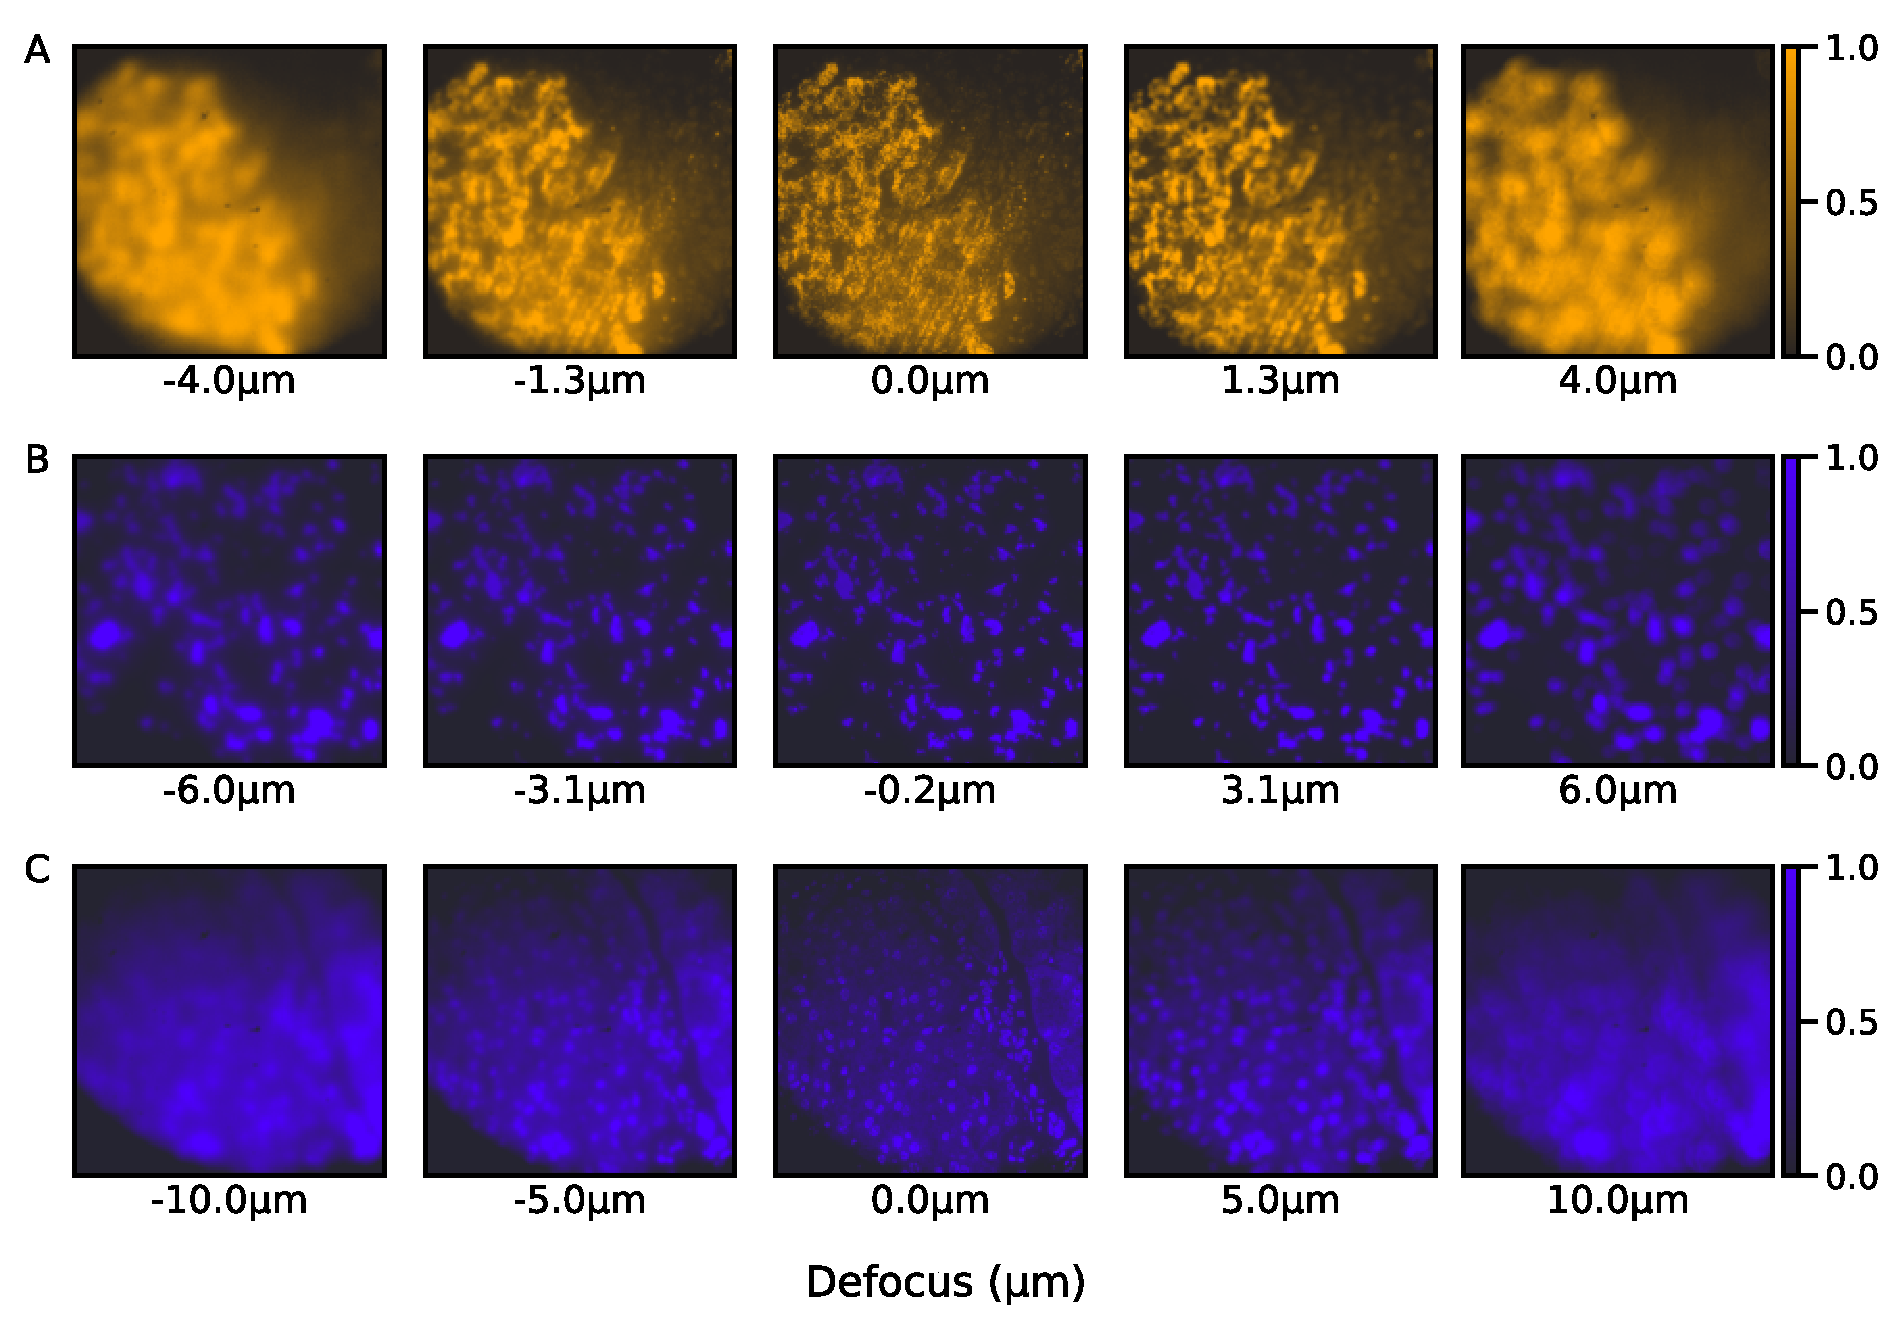
\includegraphics[width=\linewidth]{cppendix-A/figures/fig2_sweeps_v3.pdf}
    \caption{Sample FM focus sweeps.}
    \label{fig:A.2_sweeps}
\end{figure}

We then analyze the focus sweeps by applying a host of different focus measures to the data / each image in the focus sweep (Figure \ref{fig:A.3_metrics}). We get these metrics from \textcite{pertuz2013analysis}. \textcite{pertuz2013analysis} analyzed a bunch of different focus metrics to compare performance for a variety of applications. The metrics belong to different families. Explain... He concluded that "operators of the same family respond similarly to noise, contrast and window size" and that the relative performance of the focus measure operators depends highly on the imaging conditions. Here, although there is somewhat of a variety in terms of channel and scene, the imaging conditions are virtually the same. So perhaps one focus metric stands out.

% --- Fig A.3 (metrics) ---
\begin{figure}[!tbh]
    \centering
    \includegraphics[width=\linewidth]{cppendix-A/figures/fig3_metrics_v1.pdf}
    \caption{Analysis of 24 potential focus measures.}
    \label{fig:A.3_metrics}
\end{figure}

To assess the relative performance of each focus metric, we first look at how far off metrics are from picking in-focus image. This is close to 0 but not necessarily 0 because we don't want to assume that we started exactly in focus. So we take the mode from all metrics. Black means it hit peak, red means it was off with more red meaning more off. We see that Laplacian metrics have a bias towards overfocused images. We can eliminate HISE, CURV, ACMO, as well. GRAS is just GRAE (squared) and GRAT is basically identical to SFRQ for a default threshold of 0. We're not going to experiment with different threshold values as that's too much. Note that variance of Laplacian, used by Odemis, is LAPV. Now we have a number of candidate metrics. Next we can look at tougher focusing conditions and look for where methods might diverge.



 % --- Table A.1 (references) ---
\begin{table}[!tbh]
    \centering
    \caption{Reference list for focus measures.}
    \begin{tabular}{@{}llr@{}}
    \toprule
    & Focus measure & Reference \\
    \arrayrulecolor{black!30}\midrule
    \texttt{ACMO} & Absolute central moment & \cite{shirvaikar2004optimal} \\
    \texttt{BREN} & Brenner's focus measure & \cite{santos1997evaluation} \\
    \texttt{CURV} & Image curvature & \cite{helmli2001adaptive} \\
    \texttt{GDER} & Gaussian derivative & \cite{geusebroek2000robust} \\
    \texttt{GLVA} & Gray-level variance & \cite{krotkov1986range} \\
    \texttt{GLVV} & Gray-level local variance & \cite{pech2000diatom} \\
    \texttt{GRAE} & Energy of gradient & \cite{subbarao1992focusing} \\
    \texttt{GRAT} & Thresholded gradient & \cite{santos1997evaluation} \\
    \texttt{GRAS} & Squared gradient & \cite{eskicioglu1995image} \\
    \texttt{HELM} & Helmli's measure & \cite{helmli2001adaptive} \\
    \texttt{HISE} & Histogram entropy & \cite{krotkov1986range} \\
    \texttt{LAPE} & Energy of Laplacian & \cite{subbarao1992focusing} \\
    \texttt{LAPM} & Modified Laplacian & \cite{nayar1990shape} \\
    \texttt{LAPV} & Variance of Laplacian & \cite{pech2000diatom} \\
    \texttt{LAPD} & Diagonal Laplacian & \cite{thelen2008improvements}  \\
    \texttt{SFIL} & Steerable filters-based & \cite{minhas20093d} \\
    \texttt{SFRQ} & Spatial frequency & \cite{eskicioglu1995image} \\
    \texttt{TENG} & Tenegrad & \cite{krotkov1986range} \\
    \texttt{TENV} & Tenengrad variance & \cite{pech2000diatom} \\
    \texttt{VOLA} & Vollat's correlation-based & \cite{santos1997evaluation} \\
    \arrayrulecolor{black}\bottomrule
    \end{tabular}
\end{table}
